\subsubsection*{Registrierungsschlüssel \faKey}

Über den Knopf \jinline|Edit| kann der Administrator den Registrierungsschlüssel ändern, um kompromittierte Schlüssel zu ersetzen (siehe Abbildung~\vref{fig:AdminEditRegKeyImplement}). 
Über den Knopf \jinline|Show|\xspace kann der aktuelle Registrierungsschlüssel ausgelesen werden. 

\begin{figure}[h]
	\centering
	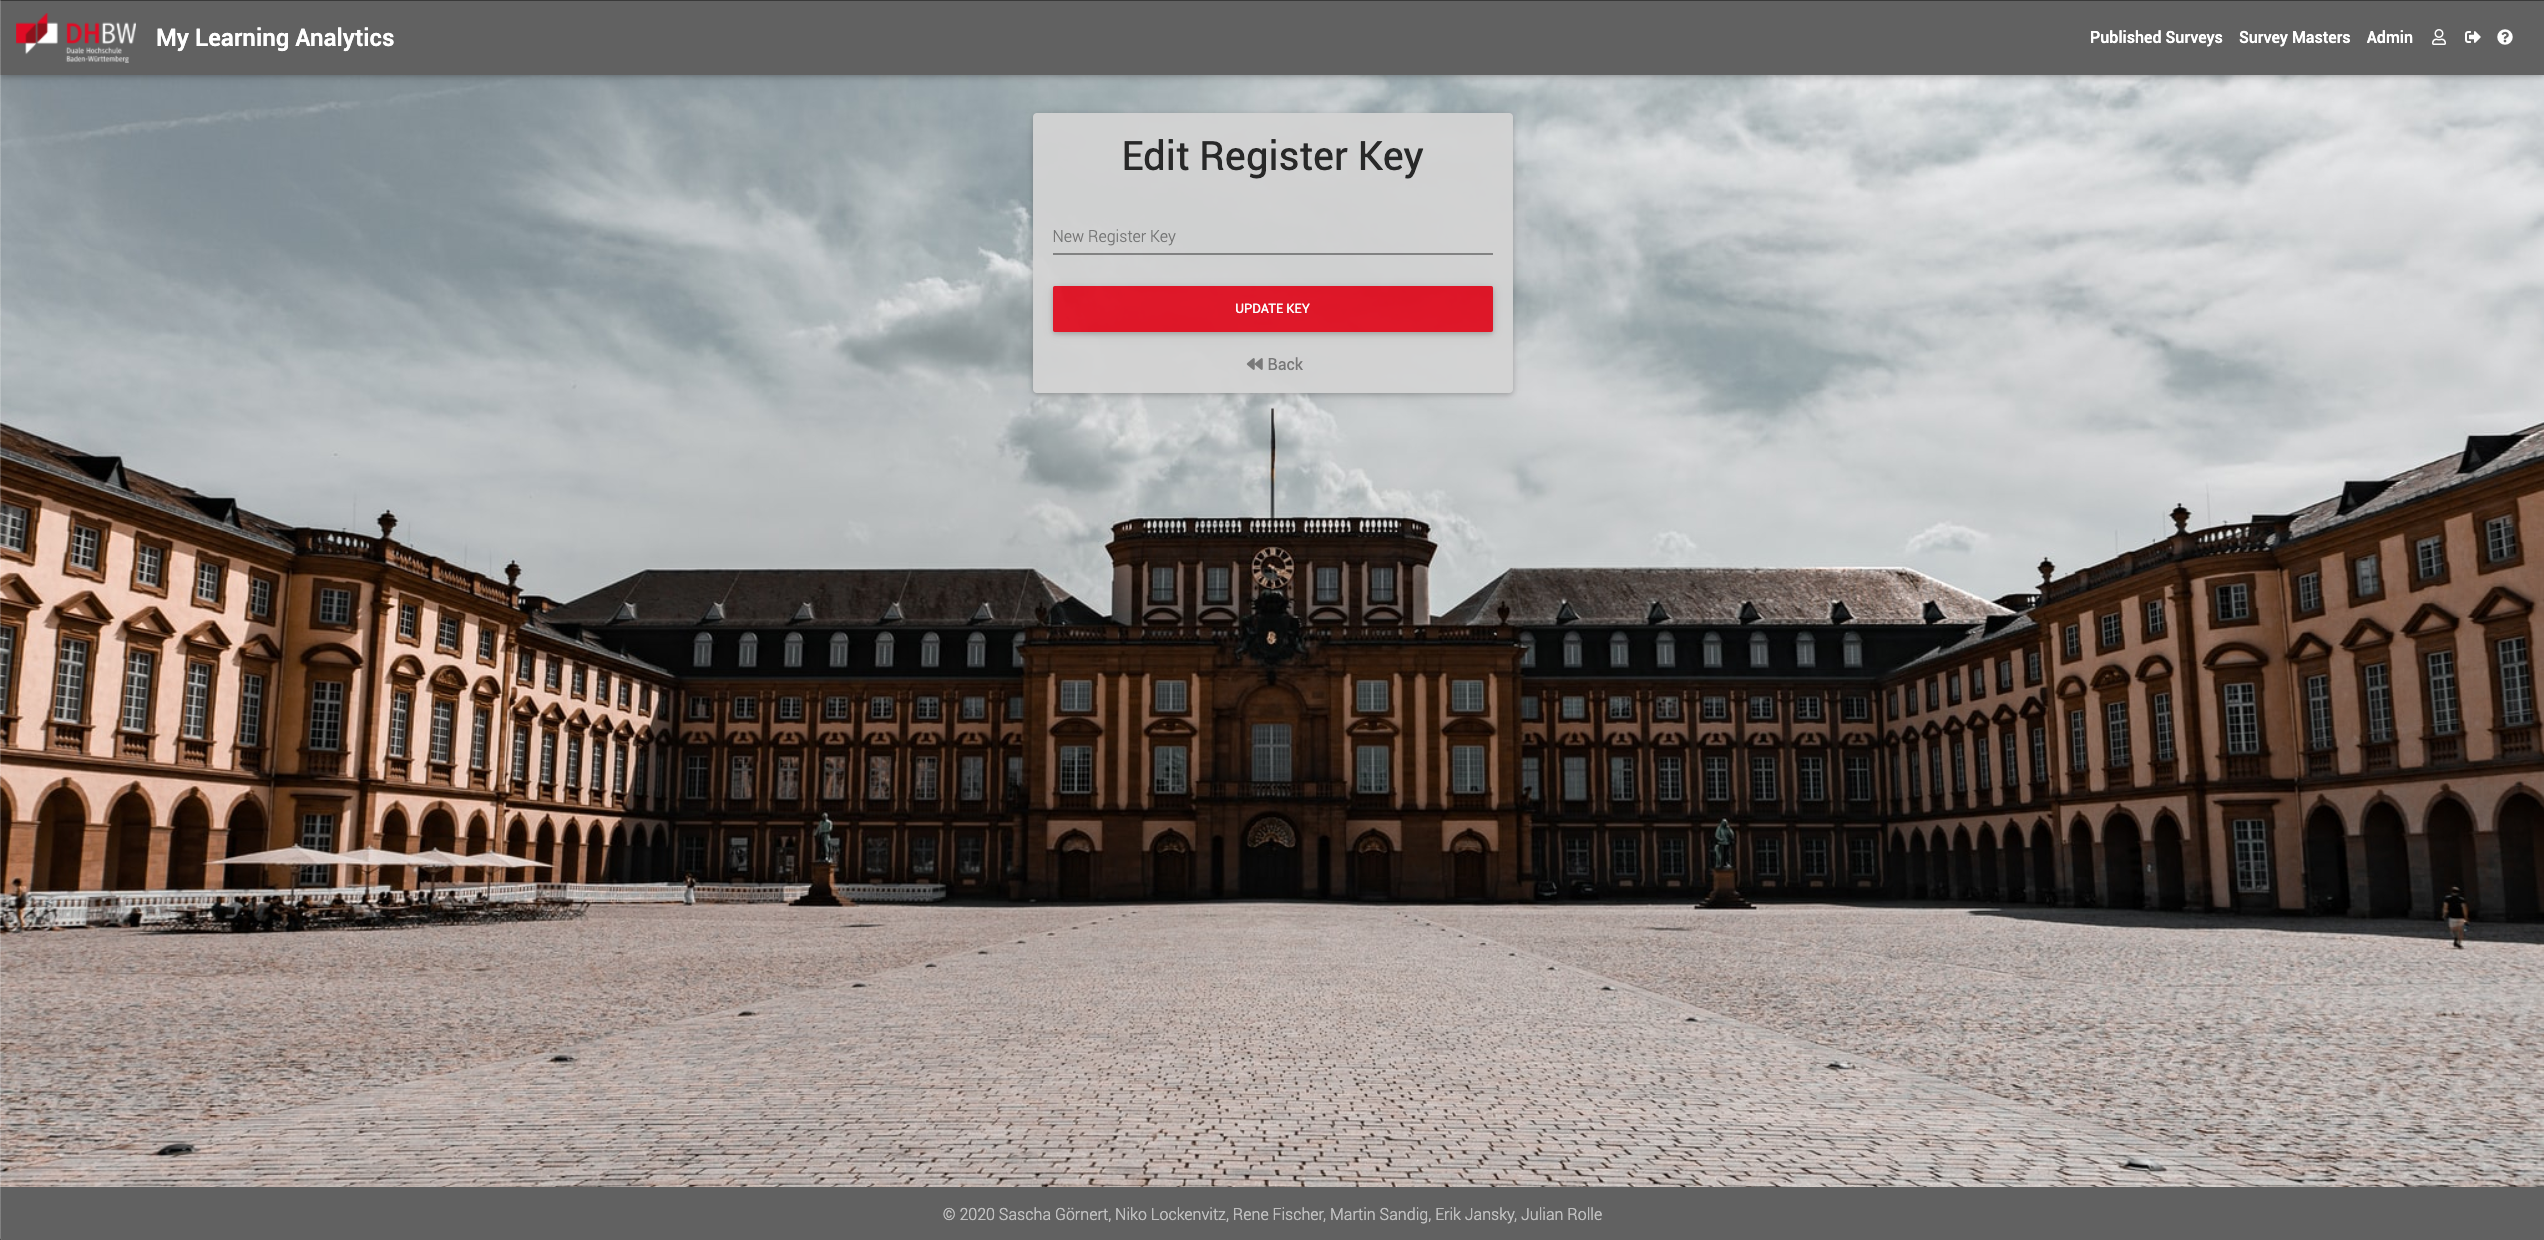
\includegraphics[width=0.95\textwidth, keepaspectratio]{img/client/EditSurveyMasterKey.png}
	\captionsetup{justification=centering, format=plain}
	\caption[\acl{UI}: Setzen eines neuen Registrierungsschlüssels]{\acl{UI}: Setzen eines neuen Registrierungsschlüssels \\ \quelleScreenshot}
	\label{fig:AdminEditRegKeyImplement}
\end{figure}
